% Notes on Magnus project
% Created 01/08/19 by A.T. (tropiano.4@osu.edu)
% Update: transitioning these notes into a draft of the eventual paper

\documentclass[preprintnumbers,floatfix,aps,prc,preprint,nofootinbib]{revtex4-1}

% Packages
\usepackage{amsmath}
\usepackage{amsfonts}
\usepackage{amssymb}
\usepackage{bm}
\usepackage[font=small,skip=0pt]{caption} % For captions on figures and tables
\usepackage{cellspace}
\usepackage{color}
\usepackage{enumerate}
\usepackage{epsfig}
\usepackage[figuresright]{rotating}
\usepackage{float}
\usepackage{hyperref} % For clickable links to sections within table of contents
\usepackage{graphicx}
\graphicspath{{Figures/}} % Setting the graphics path
\usepackage{physics} % For bra-ket notation
\usepackage{siunitx}

\newcommand{\eps}{\varepsilon}


\begin{document}


%%%%%%%%%%%%%%%%%%%%%%%%%%%%%%%%%%%%%%%%%%%%%%%%%%%%%%%%%%%%%%%%%%%%%%%%%
\title{Exploring the Magnus expansion and the in-medium similarity renormalization group}


\author{A.~J.~Tropiano$^{1}$, S.~K.~Bogner$^{2}$, R.~J.~Furnstahl$^{1}$}

\affiliation{
$^1$\mbox{Department of Physics, The Ohio State University, Columbus, OH 43210, USA}  \\
$^2$\mbox{National Superconducting Cyclotron Laboratory and Department of Physics and Astronomy,}  \\
    \mbox{Michigan State University, East Lansing, MI 48824, USA}}

\date{\today}

\begin{abstract}
\noindent{-- Test Magnus expansion SRG implementation on LO NN potential at high $\Lambda$. (Define SRG or IMSRG acronym in abstract.)}
\\
-- High $\Lambda$ leads to spurious bound states in spin triplet channels.
\\
-- Decouple spurious bound state(s) by using two approaches within the Magnus implementation to drive the Hamiltonian to band-diagonal, unitarily equivalent form.
\\
-- One choice of generator where the deep bound state is decoupled outside low-momentum and another where it is shifted to low-momentum.
\\
-- Deep bound state corrupts low-momentum physics.
\\
-- Connection to IMSRG intruder state problem.
\\
-- Confirm unitarity of Hamiltonian by evaluation of deuteron observables.
\\
-- Lastly, study operator evolution.
\end{abstract}


\maketitle

\newpage


%%%%%%%%%%%%%%%%%%%%%%%%%%%%%%%%%%%%%%%%%%%%%%%%%%%%%%%%%%%%%%%%%%%%%%%%%
\section{Introduction}
\label{sec:intro}


\noindent{-- In recent years \textit{ab initio} methods have made strides in nuclear structure and reactions.}
\\
-- Realistic binding energies starting from NN and 3N forces have been calculated for many medium mass nuclei using different many-body methods.
\\
-- The in-medium similarity renormalization group (IMSRG) is one such method \cite{Hergert:2015awm, Hergert:2016iju}.
\\
-- The IMSRG separates energy scales in the nuclear Hamiltonian by decoupling the reference state from excited states to band- or block-diagonal form.
\\
-- One can use the decoupled Hamiltonian to solve the many-body Sch{\"o}dinger equation extracting specific eigenvalues and eigenstates which qualifies the IMSRG as an \textit{ab initio} method.
\\


\noindent{-- The IMSRG procedure requires solving a system of nonlinear, coupled differential equations which can often be stiff necessitating a high-order ODE solver.}
\\
-- In principle, the decoupled Hamiltonian (or any operator) is unitarily equivalent but the numerical error of solving the ODE can lead to error on observable quantities.
\\
-- Furthermore, the model spaces for IMSRG calculations can be extremely large.
\\
-- Evolving several operators is often impossible due to memory restrictions in storing several operators.
\\


\noindent{-- A variant of the IMSRG that utilizes the Magnus expansion can overcome these limitations.}
\\
-- We will refer to this as the Magnus implementation or simply Magnus.
\\
-- The Magnus solves for the unitary transformation directly whereas the IMSRG applies the transformation indirectly in steps of the differential flow equation.
\\
-- From the form of the transformation, the numerical error leaves the unitarity of the evolved Hamiltonian un-affected.
\\
-- By explicitly solving for the transformation, one can evolve several operators.
\\
-- The Magnus implementation has become a standard technique in IMSRG calculations as studies have targeted observables such as radii, electromagnetic moments and transitions, etc., requiring consistently evolved operators.
\\


\noindent{-- We test the Magnus implementation on chiral non-local NN potentials in free-space for several EFT cutoffs.}
\\
-- At high cutoffs, spin triplet channels feature spurious, deeply bound states from the strong, repulsive tensor force \cite{Nogga:2005hy}.
\\
-- These bound states are features of high-momentum physics and lie outside the range of the EFT.
\\
-- However, potentials with deeply bound states have shown sensitivity to SRG transformations \cite{Glazek:2008pg, Wendt:2011qj}.
\\
-- Details of the SRG transformation can cause the spurious bound state(s) to corrupt the low-momentum physics.
\\
-- An analogous problem occurs in IMSRG calculations for systems with intruder states where the intruder state can shift to the energy scale of the reference state in valence space.
\\
-- This severely distorts low-energy properties such as the ground state wave function.
\\
-- It is not understood how the IMSRG procedure evolves intruder state systems.
\\
-- Due to the prominence of the Magnus in IMSRG, one must first understand if the Magnus approach matches the typical approach for difficult systems before investigating the intruder state problem.
\\
-- NN potentials with spurious bound states offer a good test laboratory for the Magnus implementation to better understand if the Magnus is equivalent to the SRG approach. 
\\


\noindent{-- The past decade has seen a tremendous increase in the number of chiral NN potentials.}
\\
-- Interactions can now be built up to N5LO and feature several different regularization schemes.
\\
-- A natural question is to ask whether the SRG decouples these potentials in the same way.
\\
-- There is evidence of universal, low-momentum matrix elements as seen from evolving different potentials with SRG transformations or $V_{low~k}$ \cite{Dainton:2013axa}.
\\
-- There has also been renewed interest in chiral potentials at high-cutoffs but for a locally regulated potential \cite{Tews:2018sbi}.
\\
-- Given the growing number of chiral interactions, it would be interesting to re-examine these areas from an SRG standpoint.
\\
-- However, we would like to focus on a fixed comparison of the SRG and the Magnus approach as a first test, and therefore only consider evolving non-local LO NN potentials at various cutoffs.
\\
-- We leave the other areas as topics for future studies.
\\


\noindent{-- The rest of the paper is organized as follows:}
\\
-- In Sec. \ref{sec:formalism} we review the formalism of the SRG and the Magnus implementation emphasizing the major advantages of the Magnus.
\\
-- In Sec. \ref{sec:results} we test the Magnus implementation on high-cutoff NN potentials.
\\
-- We briefly review the SRG results for the same set of bare interactions and compare Magnus to SRG results.
\\
-- With the Magnus evolved operators, we calculate several observables and explore operator evolution.
\\
-- Lastly, we summarize our results in Sec. \ref{sec:conclusion}.
\\
-- We discuss the implications for the Magnus expansion within the IMSRG.


%%%%%%%%%%%%%%%%%%%%%%%%%%%%%%%%%%%%%%%%%%%%%%%%%%%%%%%%%%%%%%%%%%%%%%%%%
\section{Formalism}
\label{sec:formalism}


\noindent{\textbf{SRG formalism}}
\\
-- In this section we describe the SRG in the context of decoupling any operator.
\\
-- The SRG decouples low- and high-momentum scales by applying a continuous unitary transformation $U(s)$ where $s=0 \rightarrow \infty$ is the flow parameter.
\\
-- The `dressed' or evolved operator is given by
%
\begin{eqnarray}
  \label{eq:srg_operator}
  O(s) = U(s) O(0) U^{\dagger}(s),
\end{eqnarray}
%
where $O(0)$ corresponds to the `bare' operator.
\\
-- Because $U(s)$ is unitary, the observables of the operator are preserved.
\\
-- In practice, the unitary transformation U(s) is not explicitly solved for; the evolved operator is given by a differential flow equation which is obtained by taking the derivative of Eqn. (\ref{eq:srg_operator}),
%
\begin{eqnarray}
  \label{eq:srg_flow}
  \frac{dO(s)}{ds} = [\eta(s), O(s)],
\end{eqnarray}
%
where $\eta(s)=\frac{dU(s)}{ds} U^{\dagger}(s) = -\eta^{\dagger}(s)$ is the anti-hermitian SRG generator.
\\
-- The generator is defined as a commutator,
%
\begin{eqnarray}
  \label{eq:srg_generator}
  \eta(s) = [G, H(s)],
\end{eqnarray}
%
where $G$ specifies the type of flow or form of the decoupled operator.
\\
-- To drive the operator to band-diagonal form, set $G=H_D(s)$, the diagonal of the Hamiltonian.
\\
-- This choice was implemented by Wegner in condensed matter physics \cite{Wegner:1994ab}.
\\
-- For notational convenience, we write the Wegner choice without the $s$ dependence in the rest of the paper.
\\
-- In a similar option used in nuclear physics, $G$ is set to the relative kinetic energy, $T_{rel}$, which also drives to band-diagonal form.
\\
-- In this paper, we consider both choices.
\\
-- Generally the flow equation (\ref{eq:srg_flow}) is solved up to some finite value of $s$ with a high-order ODE solver.
\\
-- It is convenient to define $\lambda \equiv s^{-1/4}$ which roughly measures the width of the diagonal in the decoupled operator.
\\

\noindent{\textbf{Magnus expansion formalism}}
\\
-- We now consider the Magnus implementation.
\\
-- Mathematically speaking, the Magnus expansion is a method for solving an initial value problem associated with a linear ordinary differential equation (ODE).
\\
-- Formal details of the Magnus expansion are discussed in \cite{Blanes:2009ab}.
\\
-- We will introduce the Magnus expansion in the context of SRG evolving any operator.
\\
-- In an intermediate step in deriving Eqn. (\ref{eq:srg_flow}), we have a linear ODE for $U(s)$,
%
\begin{eqnarray}
  \label{eq:unitary_trans}
  \frac{dU(s)}{ds} = \eta(s) U(s).
\end{eqnarray}
%
-- Magnus showed that one can solve the following equation with a solution $U(s)=e^{\Omega(s)}$ where $\Omega(s)$ is expanded as a power series, $\sum_{n}^{\infty} \Omega_n$ (referred to as the Magnus expansion or Magnus series).
\\
-- The terms of the series are given by integral expressions involving $\eta(s)$ (again, see \cite{Blanes:2009ab, Magnus:1954zz} for details).
\\
-- For our case, we focus on the formally exact derivative of $\Omega(s)$,
%
\begin{eqnarray}
  \label{eq:magnus_omega}
  \frac{d\Omega(s)}{ds} = \sum_{k=0}^{\infty} \frac{B_k}{k!} ad_{\Omega}^{k}(\eta),
\end{eqnarray}
%
where $B_k$ are the Bernoulli numbers, $ad_{\Omega}^{0}(\eta)=\eta(s)$, and $ad_{\Omega}^{k}(\eta)=[\Omega(s),ad_{\Omega}^{k-1}(\eta)]$.
\\
-- We integrate this differential equation to find $\Omega(s)$ and evaluate the unitary transformation directly.
\\
-- Then the evolved operator can be evaluated with the BCH formula:
%
\begin{eqnarray}
  \label{eq:bch}
  O(s) = e^{\Omega(s)} O e^{-\Omega(s)} = \sum_{k=0}^{\infty} \frac{1}{k!} ad_{\Omega}^{k}(O).
\end{eqnarray}
%
-- As $k \rightarrow \infty$ in both sums in Eqns. (\ref{eq:magnus_omega}) and (\ref{eq:bch}) the Magnus transformation matches the SRG transformation.
\\
-- We investigate several truncations $k_{max}$ in Eqn. (\ref{eq:magnus_omega}) and take many terms, $k_{max} \sim 25$, in Eqn. (\ref{eq:bch}).
\\
\textcolor{red}{-- Here or earlier (for the following bullets)? Better to motivate the Magnus in the introduction or easier to explain given mathematical detail?}
\\
-- There are significant advantages in the Magnus implementation.
\\
-- In the typical approach, the numerical error associated with solving the flow equation affects the accuracy of the observables for the evolved operator.
\\
-- Therefore, one must use a high-order ODE solver in integrating the flow equation (\ref{eq:srg_flow}).
\\
-- In the Magnus implementation, unitarity is guaranteed by the form of $U(s)$; in fact, one could solve Eqn. (\ref{eq:magnus_omega}) with a simple first-order Euler step-method keeping the same observables while decoupling the operator as desired.
\\
-- This offers a decent computational speed-up by avoiding a high-order solver.
\\
-- In this paper, we demonstrate this advantage by applying the Magnus implementation using the first-order Euler step-method.
\\
-- The second major advantage involves the evolution of multiple operators.
\\
-- In many other situations, one may be interested in evolving several operators at a time.
\\
-- In the SRG procedure, we would have another set of coupled equations in Eqn. (\ref{eq:srg_flow}), drastically increasing memory usage.
\\
-- Each additional operator increases the set of equations - say $N$ equations - by another factor of $N$.
\\
-- In the Magnus, one only needs $\Omega(s)$ to consistently evolve several operators.
\\
-- We avoid the cost in memory by directly constructing $U(s)=e^{\Omega(s)}$.
\\
-- This is especially useful in IMSRG calculations where the model space can be very large.
\\
-- In the next section, we discuss results from Magnus evolved large-cutoff potentials focusing on the flow of the potential, observables, and operator evolution.


%%%%%%%%%%%%%%%%%%%%%%%%%%%%%%%%%%%%%%%%%%%%%%%%%%%%%%%%%%%%%%%%%%%%%%%%%
\section{Results}
\label{sec:results}


\noindent{\textbf{Evolution of potentials}}
\\
-- In this section, we Magnus evolve LO non-local potentials in the $^{3}S_1-^{3}D_1$ channel at cutoffs of $\Lambda=4$, $9$, and $20 \, fm^{-1}$.
\\
\textcolor{red}{-- Option: add new regularization schemes?}
\\
-- For the higher two cutoffs, the potentials have one and two spurious, deeply bound states, respectively.
\\
-- In \cite{Wendt:2011qj}, potentials at large-cutoffs were SRG evolved with $G=H_D$ and $G=T_{rel}$.
\\
-- At lower cutoffs ($\Lambda \lesssim 4 \, fm^{-1}$), potential matrix elements flowed toward a decoupled, universal form independent of $G$, that is the low-momentum matrix elements approached the same values as $\lambda \rightarrow 0$.
\\
-- However, SRG evolution differed for potentials featuring one or more spurious bound states.
\\
-- With one or more spurious bound states and $G=T_{rel}$, the SRG transformation shifted a spurious bound state toward the low-momentum block corrupting the low-energy physics (e.g., the deuteron wave function, phase shifts, etc.).
\\
-- For $G=H_D$, the SRG decoupled the spurious bound state outside the low-momentum block matching the flow to universal low-momentum form independent of the cutoff $\Lambda$.
\\
-- Similar behavior could be prevalent in IMSRG calculations where the choice in generator affects evolution of many-body Hamiltonians with intruder states as it does for these NN potentials in free-space SRG.
\\


\noindent{-- First, we compare Magnus to SRG evolution for large cutoff potentials with $G=H_D$ and $G=T_{rel}$.}
\\
-- Figures \ref{fig:magnus_contours_Wendt_Lamb9_Wegner} and \ref{fig:magnus_contours_Wendt_Lamb9_T} show potential matrix element evolution for three truncations in the sum of Eqn. \ref{eq:magnus_omega} up to three values of $\lambda$ with $\Lambda=9 \, fm^{-1}$.
\\
-- At this cutoff, the potential has one spurious bound state at about $-2000$ MeV.
\\
%	
\begin{figure}
  \captionsetup{singlelinecheck=false,justification=raggedright}
  \centering
  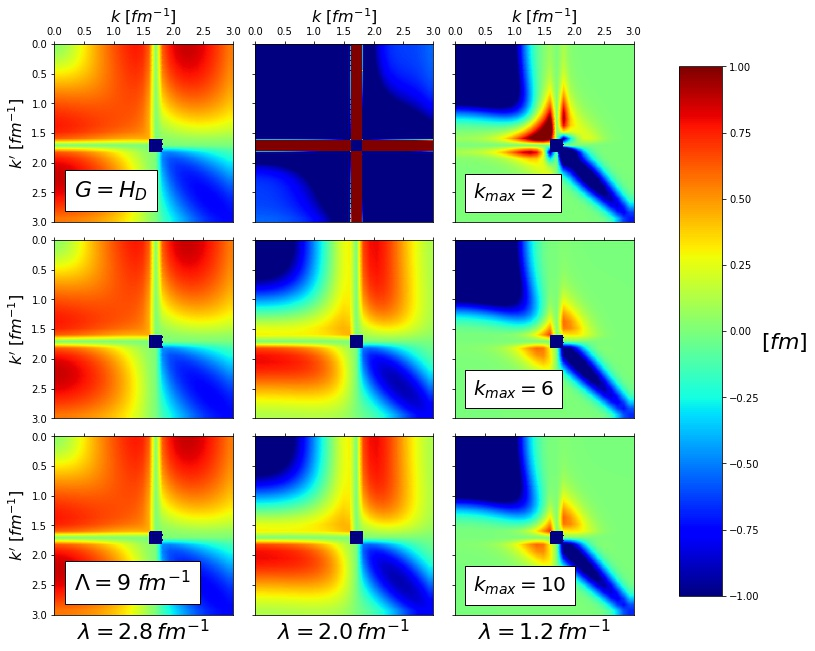
\includegraphics[width=10cm]{magnus_contours_Wendt_Lamb9_Wegner}
  \hspace*{0.05\textwidth}
  \caption{Contours of Magnus evolved $V_{\lambda}(k,k')$ with $\Lambda=9 \, fm^{-1}$ and $G=H_{D}$ for $\lambda=2.8$ (left), $2.0$ (middle), and $1.2$ (right) $fm^{-1}$ and truncations in the Magnus $k_{max}=2$ (top), $6$ (middle), and $10$ (bottom).}
  \label{fig:magnus_contours_Wendt_Lamb9_Wegner}
\end{figure}
%
\begin{figure}
  \captionsetup{singlelinecheck=false,justification=raggedright}
  \centering
  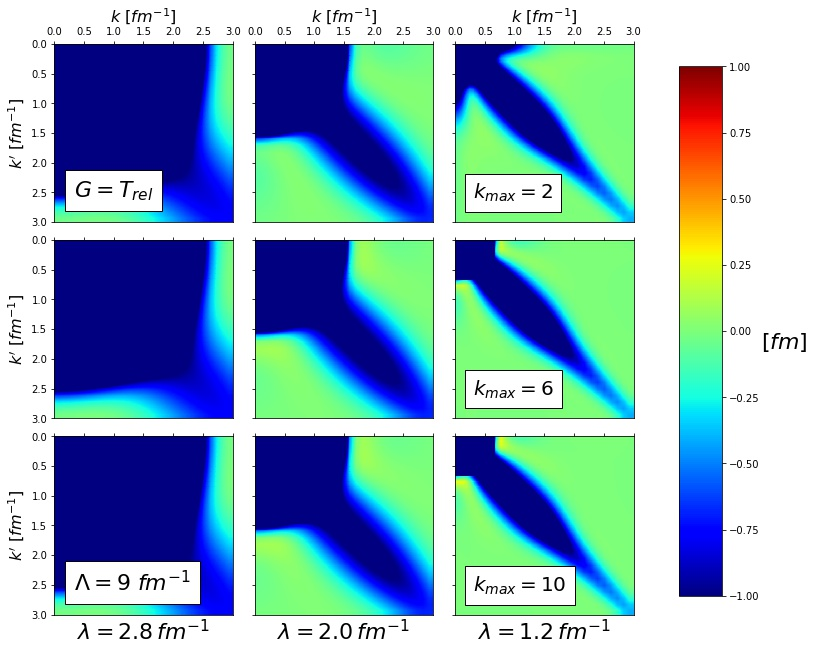
\includegraphics[width=10cm]{magnus_contours_Wendt_Lamb9_T}
  \hspace*{0.05\textwidth}
  \caption{Contours of Magnus evolved $V_{\lambda}(k,k')$ with $\Lambda=9 \, fm^{-1}$ and $G=T_{rel}$ for $\lambda=2.8$ (left), $2.0$ (middle), and $1.2$ (right) $fm^{-1}$ and truncations in the Magnus $k_{max}=2$ (top), $6$ (middle), and $10$ (bottom).}
  \label{fig:magnus_contours_Wendt_Lamb9_T}
\end{figure}
%
-- We see the same behavior with the Magnus in comparison to the SRG in \cite{Wendt:2011qj} for both generators.
\\
-- For $G=H_D$, there is a deep, blue dot in the middle of the contours at $k \approx 1.75 \, fm^{-1}$ which corresponds to the decoupled spurious bound state.
\\
-- We have checked other cutoffs and found that the evolved low-momentum matrix elements are independent of the cutoff $\Lambda$ implying a low-momentum, universal form.
\\
-- The only major difference in Magnus or SRG evolution for various cutoffs is where spurious bound state(s) are decoupled.
\\
-- This decoupling feature depends on the details of the starting interaction (i.e., the value of the bound state).
\\
%
\begin{figure}
  \captionsetup{singlelinecheck=false,justification=raggedright}
  \centering
  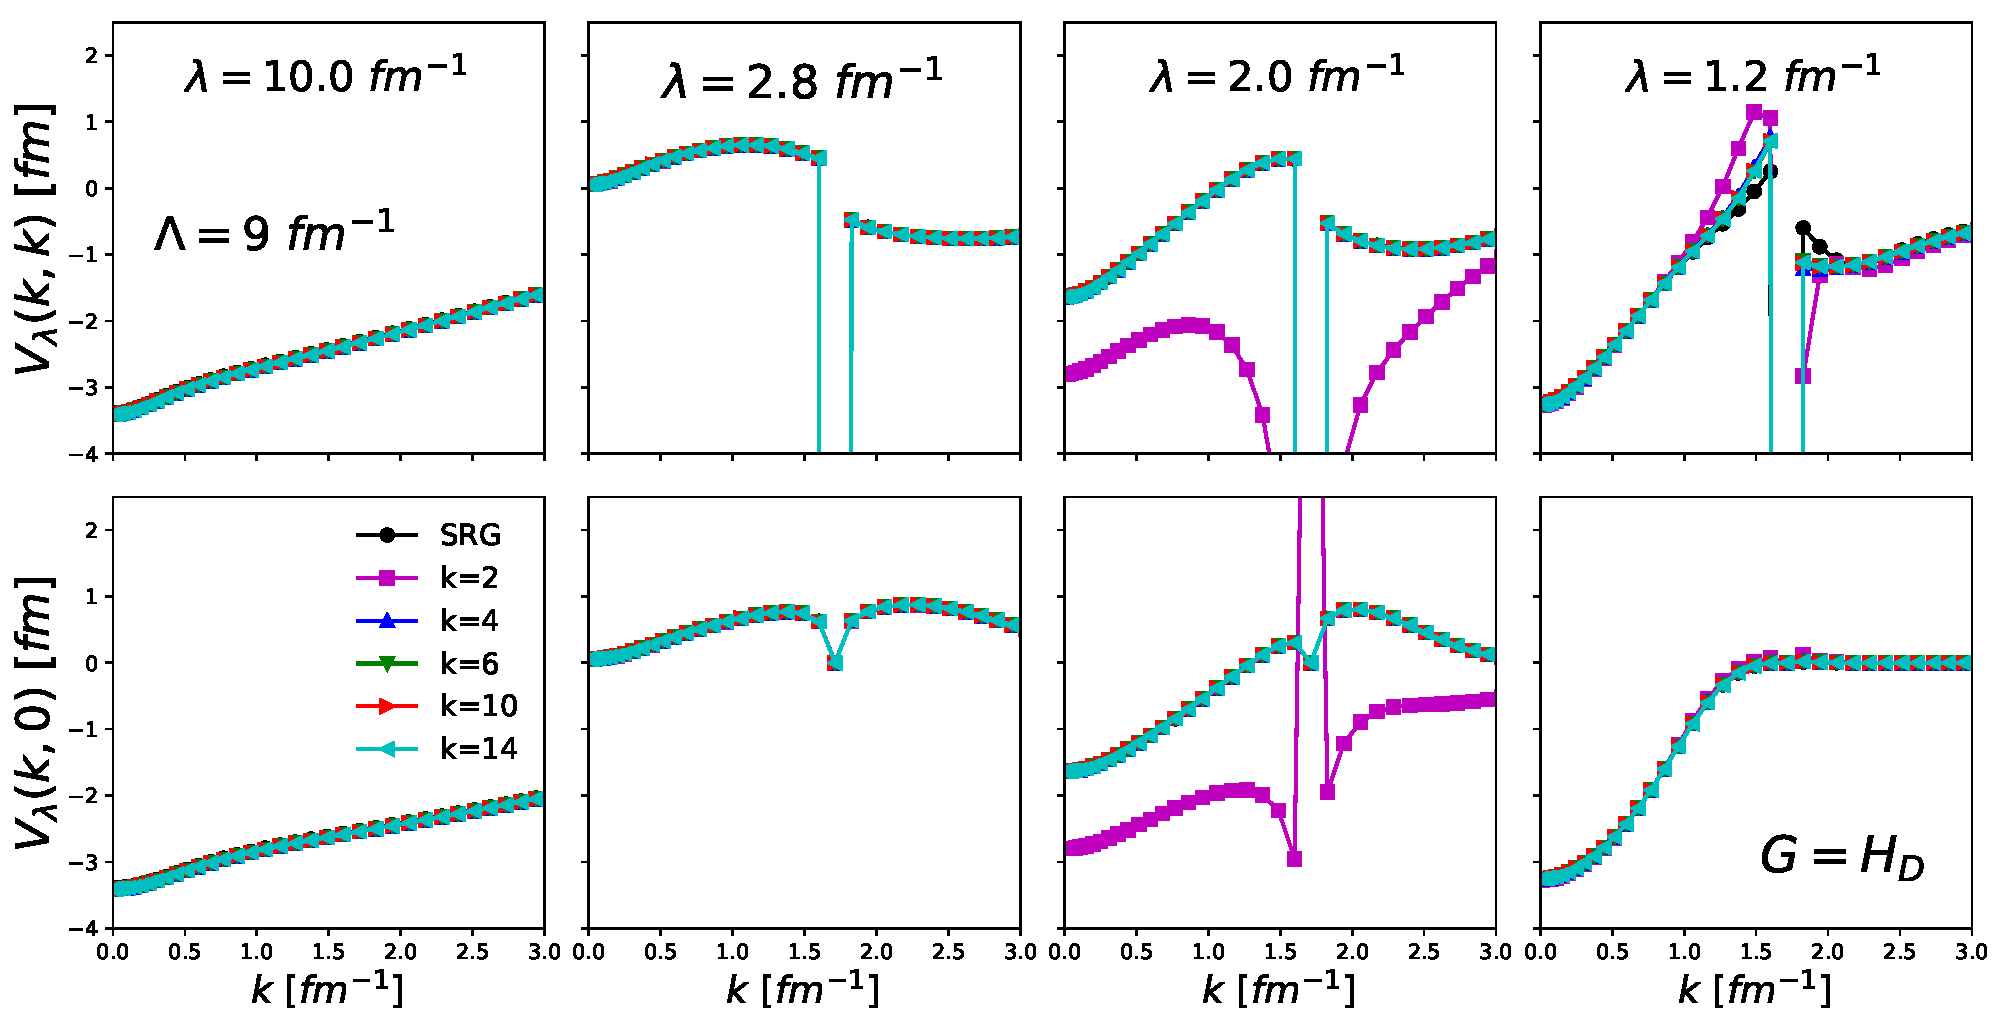
\includegraphics[width=14cm]{evolved_diags_Wendt_Lamb9_Wegner}
  \hspace*{0.05\textwidth}
  \caption{Diagonal (top row) and far off-diagonal (bottom row) matrix elements of evolved $V_{\lambda}(k,k')$ with $\Lambda=9 \, fm^{-1}$ and $G=H_{D}$ for several values of $\lambda$ and truncations in the Magnus series $k_{max}$.}
  \label{fig:evolved_diags_Wendt_Lamb9_Wegner}
\end{figure}
%
\noindent{-- Furthermore, it is dependent on the momentum mesh on which the potential is generated.}
\\
-- At $k_{max}=2$ and $\lambda=2.0 \, fm^{-1}$, we see large, positive off-diagonal values along the momentum axes where the deep bound state is decoupled.
\\
-- Solving for $\Omega(s)$ at a low truncation leads to less desirable flow, that is, the transformation $U(s)$ is not quite the same transformation as the SRG $U(s)$.
\\
-- However, the Magnus still guarantees the unitarity of $U(s)$, and we see a consistent decoupling of the spurious bound state in each row independent of $k_{max}$.
\\
-- For $G=T_{rel}$, the spurious bound state is shifted up along the diagonal, and the low-momentum block drops to extremely negative values.
\\
-- Here, the spurious bound state corrupts the low-momentum block matching the SRG evolution of different cutoffs, thus breaking universality.
\\
%
\begin{figure}
  \captionsetup{singlelinecheck=false,justification=raggedright}
  \centering
  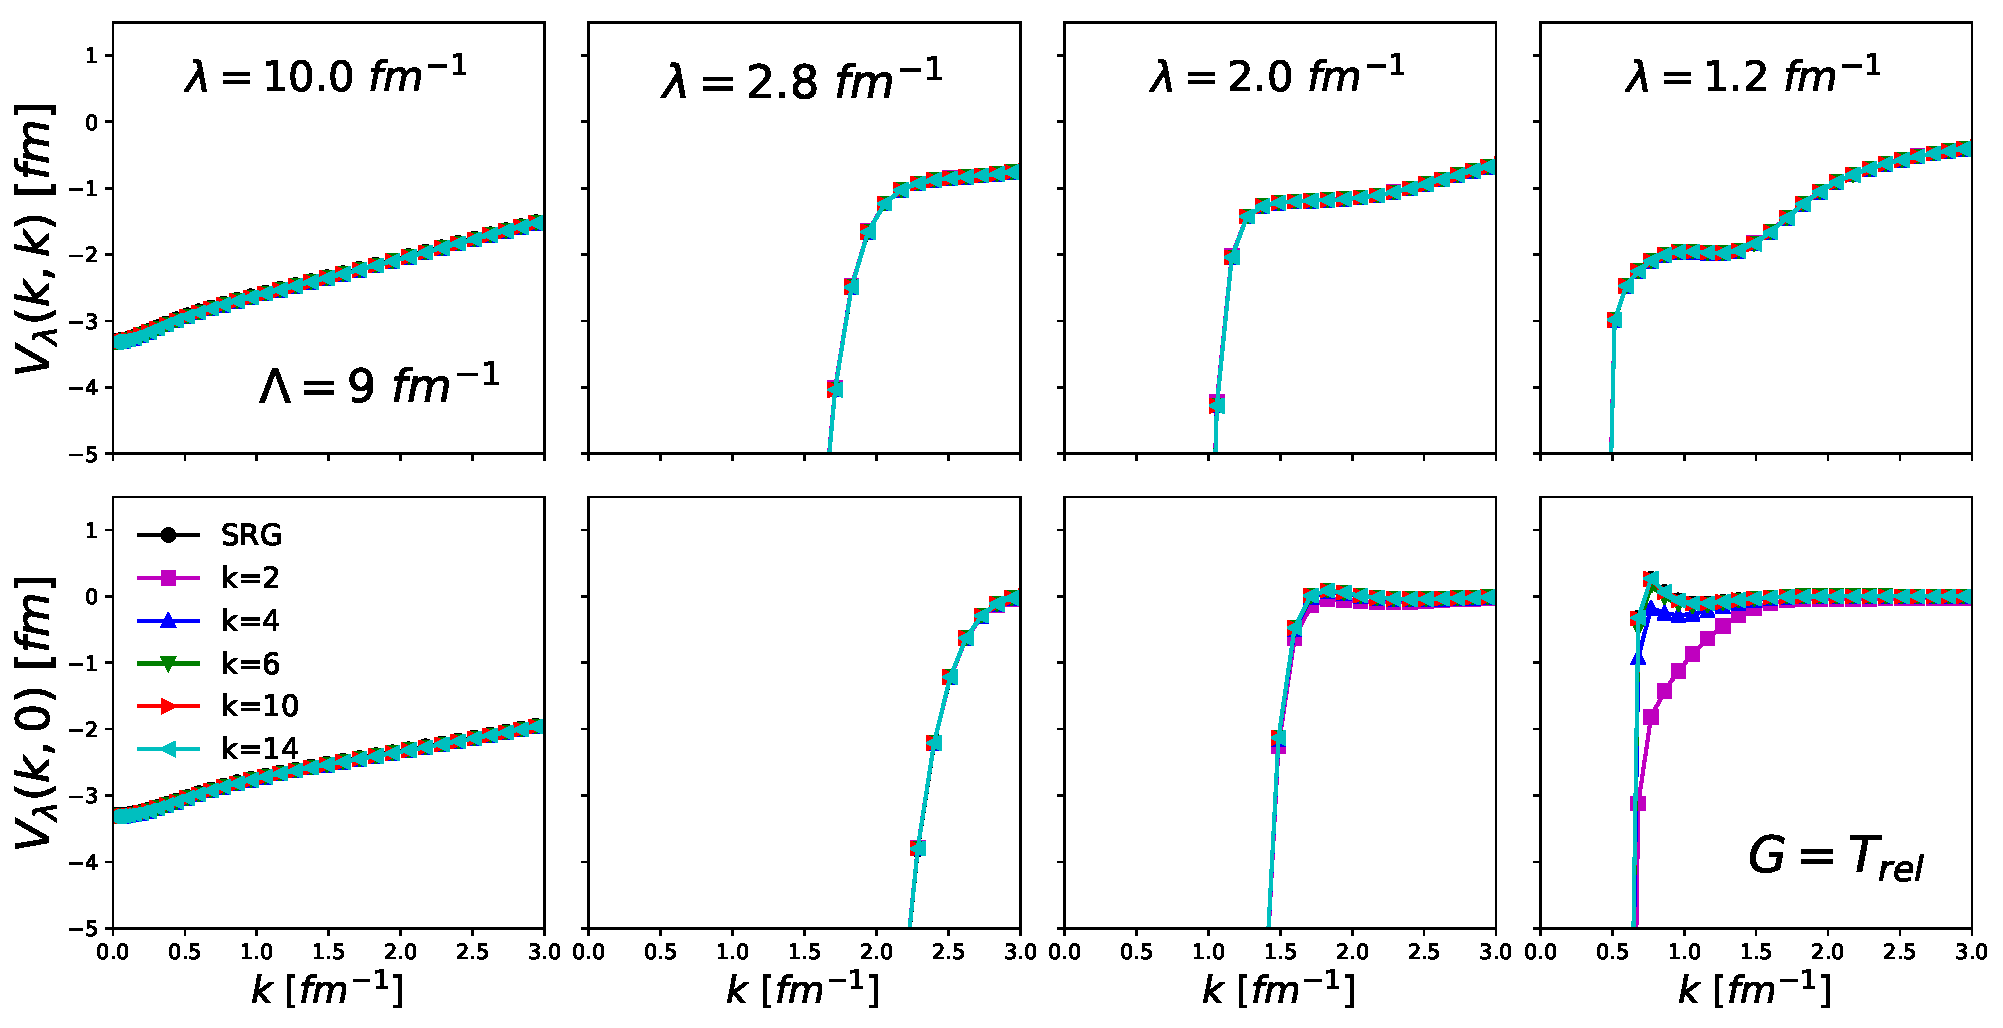
\includegraphics[width=14cm]{evolved_diags_Wendt_Lamb9_T}
  \hspace*{0.05\textwidth}
  \caption{Diagonal (top row) and far off-diagonal (bottom row) matrix elements of evolved $V_{\lambda}(k,k')$ with $\Lambda=9 \, fm^{-1}$ and $G=T_{rel}$ for several values of $\lambda$ and truncations in the Magnus series $k_{max}$.}
  \label{fig:evolved_diags_Wendt_Lamb9_T}
\end{figure}
%
\noindent{-- Figures \ref{fig:evolved_diags_Wendt_Lamb9_Wegner} and \ref{fig:evolved_diags_Wendt_Lamb9_T} show a more quantitative depiction of the evolved potentials.}
\\
-- The black dotted line corresponds to the SRG evolved potential whereas the other lines are Magnus evolved potentials for different $k_{max}$ for diagonal and far-off diagonal matrix elements of $V_{\lambda}(k,k')$.
\\
-- It is clear in these figures that the Magnus matches the SRG at $k_{max} \gtrsim 6$.
\\
-- In Figure \ref{fig:evolved_diags_Wendt_Lamb9_Wegner} the decoupled spurious bound state is seen as the large negative drop in the curves at $k \approx 1.75 \, fm^{-1}$.
\\
\textcolor{red}{-- Unnecessary?
\\
-- From applying the Magnus in several other cases, we have seen that harder potentials cause convergence issues in the Magnus expansion due to the relative size of the SRG generator $\eta(s)$.
\\
-- To avoid convergence issues we can take a smaller step-size.
\\
-- In the previous cases (and all other cases unless specified otherwise), we take $ds=10^-5$.}
\\


\noindent{\textbf{Observables}}
\\
%
\begin{table}
  \captionsetup{singlelinecheck=false,justification=raggedright}
  \caption{Relative error on the deuteron bound state energy and the root mean square of eigenvalues where $\tilde{\epsilon}$ denotes an eigenvalue of an SRG or Magnus evolved Hamiltonian for $\Lambda=9 \, fm^{-1}$ and $\lambda=1.2 \, fm^{-1}$.}
  \label{tab:energies}
  \begin{ruledtabular}
    \begin{tabular}{{>{\centering\arraybackslash}m{1.5in}>{\centering\arraybackslash}m{1in}>{\centering\arraybackslash}m{1.5in}>{\centering\arraybackslash}m{2in}}}
      $  $ & $G$ & $ |\frac{\epsilon_d-\tilde{\epsilon}_d}{\epsilon_d}| $ & $\sqrt{\frac{1}{N} \, \sum_{i}^{N} (\tilde{\epsilon}_i-\epsilon_i)^2}$   [MeV] \\
      \colrule
      SRG & $ $ & $\num{1.165e-5}$ & $\num{3.016e-4}$ \\
      Magnus, $k_{max}=2$ & $H_D$ & $\num{5.010e-10}$ & $\num{4.097e-9}$ \\
      Magnus, $k_{max}=14$ & $ $ & $\num{1.206e-11}$ & $\num{3.950e-10}$ \\ \hline
      SRG & $ $ & $\num{1.003e-4}$ & $\num{9.791e-5}$ \\
      Magnus, $k_{max}=2$ & $T_{rel}$ & $\num{7.775e-8}$ & $\num{6.376e-8}$ \\
      Magnus, $k_{max}=14$ & $ $ & $\num{7.607e-8}$ & $\num{6.359e-8}$ \\
    \end{tabular}
  \end{ruledtabular}
\end{table}
%
-- To emphasize the two major advantages of the Magnus implementation, we now consider evolved observables and operators for the remainder of the section.
\\
-- Table \ref{tab:energies} shows the relative error on the deuteron bound state energy and root mean square of all eigenvalues for several evolution cases.
\\
-- The Magnus approach preserves energies to several orders of magnitude better than the typical SRG approach.
\\
-- Again, despite the inclusion of several more terms in the sum of Eqn. \ref{eq:magnus_omega}, we see consistent errors between $k_{max}=2$ and $14$ because of the guaranteed unitarity of $U(s)=e^{\Omega(s)}$
\\
-- The errors on the Magnus energies are within the region of floating-point error whereas the SRG compounds error in solving the ODE \ref{eq:srg_flow}.
\\
-- We have also checked the phase shifts from the evolved potentials match the bare potentials in all cases for Magnus and SRG evolution.
\\ 
-- Next we show the evolved deuteron wave function for several cases.
\\
-- Figure \ref{fig:momentum_dist_Wendt_Lamb9} shows the deuteron momentum probability density, $|\phi(k)|^2$, on a semi-log scale as a function of momentum for both band-diagonal generators.
\\
-- With $G=H_D$, the evolved and un-evolved momentum distributions agree for low-momentum whereas $G=T_{rel}$ significantly distorts the distribution from the presence of the spurious bound state in the $\Lambda=9 \, fm^{-1}$ potential.
\\
-- This illustrates the advantage of the Wegner generator: the spurious bound state at high-momentum does not affect the low-momentum physics under the SRG transformation.
\\
-- In all cases of Magnus and SRG evolution, we can consistently evolve wave functions and operators to make reliable calculations of observables.
\\
-- To demonstrate this, we calculate the deuteron RMS radius and quadrupole moment with the $\Lambda=9 \, fm^{-1}$ potential using the Magnus implementation with the Wegner generator.
\\
-- The initial values of the chiral potential are $r_d = 2.022 \, fm$ and $Q_d = 0.287 \, fm^2$ compared to the experimental values $r_d^{exp} = 2.141 \, fm$ and $Q_d^{exp} = 0.286 \, fm^2$. 
\\
-- We have checked for several cases with the Magnus and found near-perfect agreement to the initial values of both observables.
\\


\noindent{\textcolor{red}{UPDATED UP TO HERE 04/03/19}}
\\
\begin{figure}
  \captionsetup{singlelinecheck=false,justification=raggedright}
  \centering
  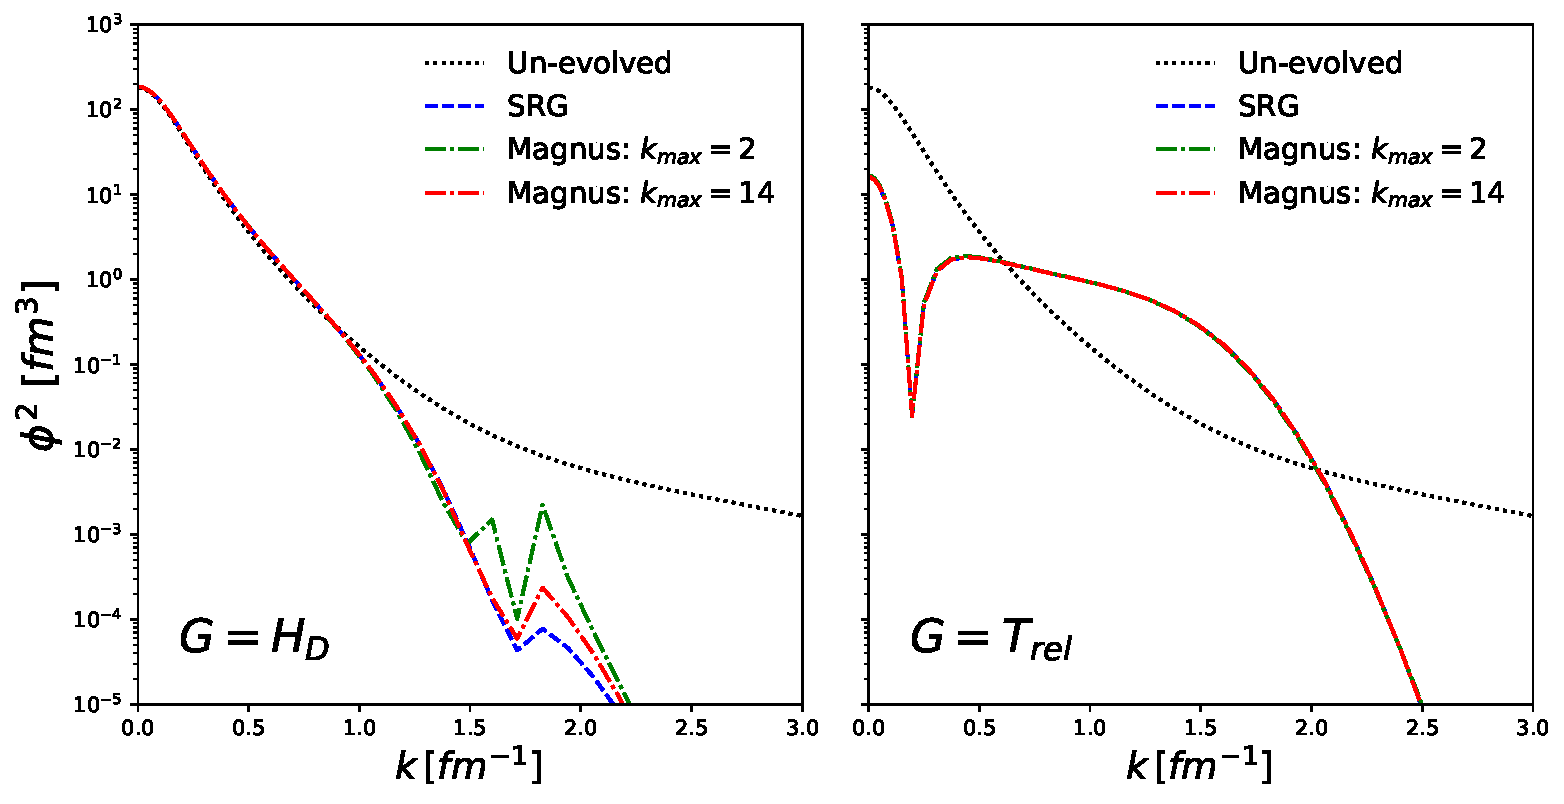
\includegraphics[width=10cm]{momentum_dist_Wendt_Lamb9}
  \hspace*{0.05\textwidth}
  \caption{Momentum probability densities of the deuteron comparing the un-evolved wavefunction (black dotted line), SRG evolved wavefunction (blue dashed line), and two Magnus evolved wavefunctions with truncations $2$ and $14$ (green and red dash-dotted lines, respectively) where $\lambda=1.2 \, fm^{-1}$. The left panel shows evolution with $G=H_{D}$ and the right with $G=T_{rel}$. Here $\Lambda=9 \, fm^{-1}$.}
  \label{fig:momentum_dist_Wendt_Lamb9}
\end{figure}
%
\noindent{-- RMS radius and quadrupole moment of deuteron.}
\\
-- Values from initial potential ($\Lambda=9 \, fm^{-1}$):
\begin{itemize}
  \item $r_d = 2.022 \, fm$ (using momentum-space derivatives)
  \item $r_d = 2.465 \, fm$ (using Fourier transforms)
  \item $Q_d = 0.287 \, fm^2$ (using momentum-space derivatives)
\end{itemize}
-- Values from standard Magnus evolved potential ($G=H_D$, $\lambda=1.2 \, fm^{-1}$, and $k_{max}=6$):
\begin{itemize}
  \item $r_d = 2.022 \, fm$ (using momentum-space derivatives)
  \item $Q_d = 0.287 \, fm^2$ (using momentum-space derivatives)s
  \item Note: we apply $U^{\dagger}(s) U(s)$ to wave function to compute unitarily equivalent observables
\end{itemize}
-- Experimental values:
\begin{itemize}
  \item $r_d = 2.141 \, fm$
  \item $Q_d = 0.286 \, fm^2$
\end{itemize}
%
\textbf{Evolution of operators}
%
\begin{figure}[H]
  \captionsetup{singlelinecheck=false,justification=raggedright}
  \centering
  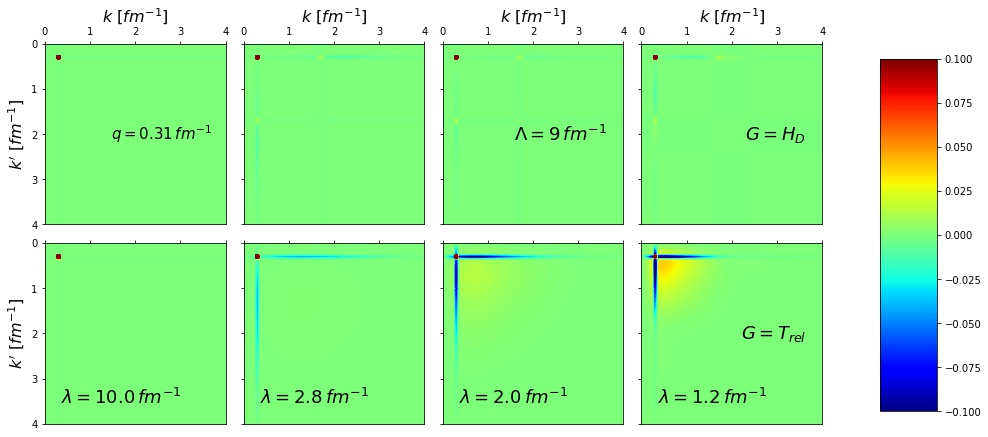
\includegraphics[width=14cm]{momentum_proj_operator_contours_q0,31_magnus_Wendt_Lamb9}
  \hspace*{0.05\textwidth}
  \caption{Matrix elements of $\mel{k}{a^{\dagger}_q a_q}{k'}$ Magnus evolving in $\lambda$ right to left with $G=H_D$ (top) and $G=T_{rel}$ (bottom). Here $q=0.31 \, fm^{-1}$, $\Lambda=9 \, fm^{-1}$, and $k_{max}=6$.}
  \label{fig:momentum_proj_operator_contours_q0,31_magnus_Wendt_Lamb9}
\end{figure}
%
\begin{figure}[H]
  \captionsetup{singlelinecheck=false,justification=raggedright}
  \centering
  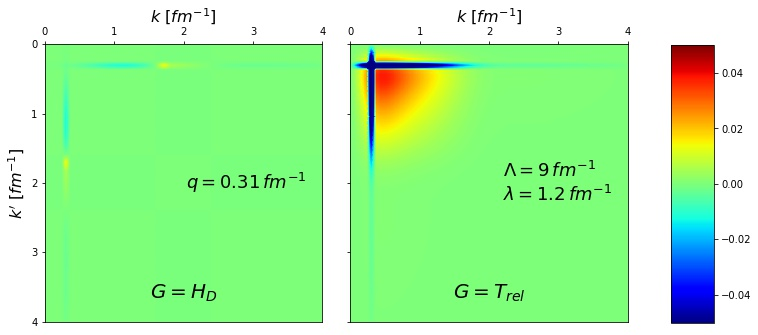
\includegraphics[width=10cm]{momentum_proj_difference_q0,31_magnus_Wendt_Lamb9}
  \hspace*{0.05\textwidth}
  \caption{Difference in evolved and bare matrix elements of $\mel{k}{a^{\dagger}_q a_q}{k'}$ Magnus evolving to $\lambda=1.2 \, fm^{-1}$ right to with $G=H_D$ (left) and $G=T_{rel}$ (right). Here $q=0.31 \, fm^{-1}$, $\Lambda=9 \, fm^{-1}$, and $k_{max}=6$.}
  \label{fig:momentum_proj_operator_difference_q0,31_magnus_Wendt_Lamb9}
\end{figure}
%
\begin{figure}[H]
  \captionsetup{singlelinecheck=false,justification=raggedright}
  \centering
  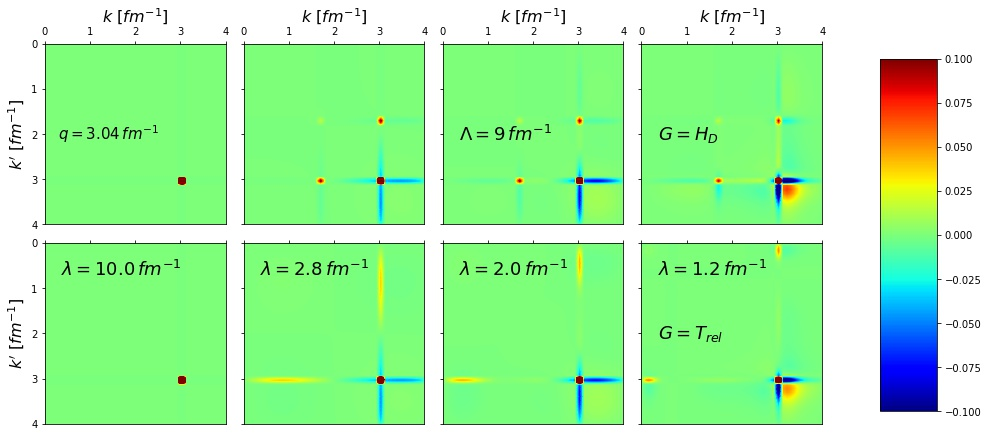
\includegraphics[width=14cm]{momentum_proj_operator_contours_q3,04_magnus_Wendt_Lamb9}
  \hspace*{0.05\textwidth}
  \caption{Matrix elements of $\mel{k}{a^{\dagger}_q a_q}{k'}$ Magnus evolving in $\lambda$ right to left with $G=H_D$ (top) and $G=T_{rel}$ (bottom). Here $q=3.04 \, fm^{-1}$, $\Lambda=9 \, fm^{-1}$, and $k_{max}=6$.}
  \label{fig:momentum_proj_operator_contours_q3,04_magnus_Wendt_Lamb9}
\end{figure}
%
\begin{figure}[H]
  \captionsetup{singlelinecheck=false,justification=raggedright}
  \centering
  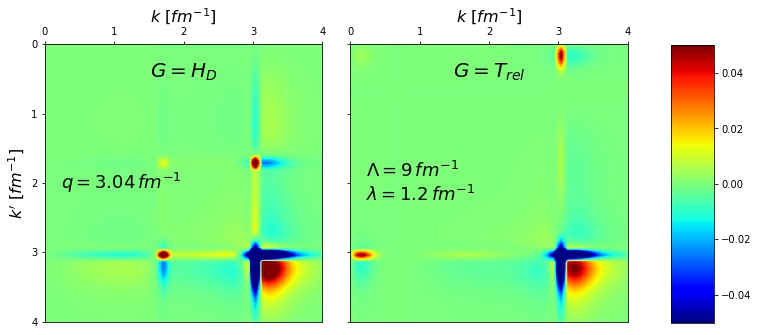
\includegraphics[width=10cm]{momentum_proj_difference_q3,04_magnus_Wendt_Lamb9}
  \hspace*{0.05\textwidth}
  \caption{Difference in evolved and bare matrix elements of $\mel{k}{a^{\dagger}_q a_q}{k'}$ Magnus evolving to $\lambda=1.2 \, fm^{-1}$ with $G=H_D$ (left) and $G=T_{rel}$ (right). Here $q=3.04 \, fm^{-1}$, $\Lambda=9 \, fm^{-1}$, and $k_{max}=6$.}
  \label{fig:momentum_proj_operator_difference_q3,04_magnus_Wendt_Lamb9}
\end{figure}
%
\begin{figure}[H]
  \captionsetup{singlelinecheck=false,justification=raggedright}
  \centering
  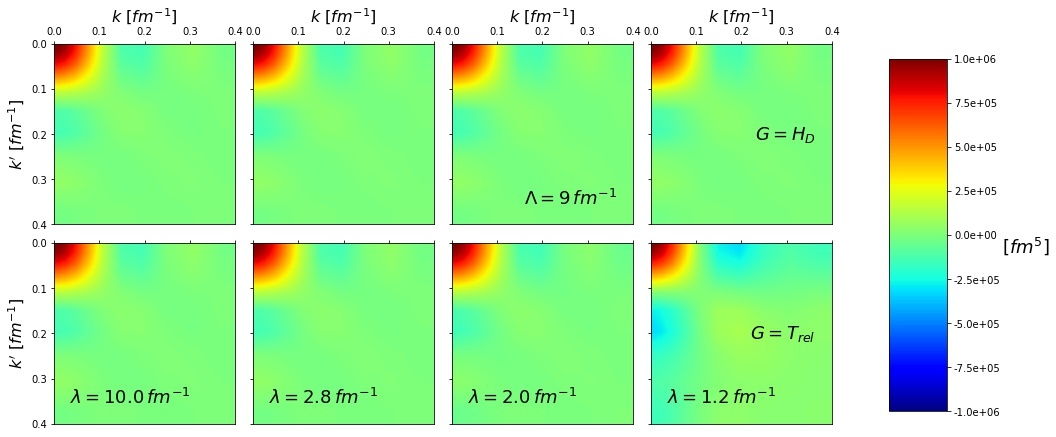
\includegraphics[width=14cm]{r2_operator_contours_magnus_Wendt_Lamb9}
  \hspace*{0.05\textwidth}
  \caption{Matrix elements of $\mel{k}{r^2}{k'}$ Magnus evolving in $\lambda$ right to left with $G=H_D$ (top) and $G=T_{rel}$ (bottom). Here $\Lambda=9 \, fm^{-1}$ and $k_{max}=6$.}
  \label{fig:r2_operator_contours_srg_Wendt_Lamb9}
\end{figure}
%
\begin{figure}[H]
  \captionsetup{singlelinecheck=false,justification=raggedright}
  \centering
  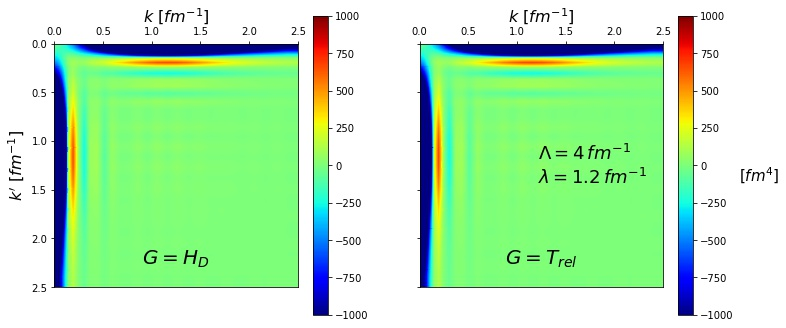
\includegraphics[width=10cm]{r2_difference_magnus_Wendt_Lamb4}
  \hspace*{0.05\textwidth}
  \caption{Difference in evolved and bare matrix elements of $\mel{k}{r^2}{k'}$ Magnus evolving to $\lambda=1.2 \, fm^{-1}$ with $G=H_D$ (left) and $G=T_{rel}$ (right). Here $\Lambda=4 \, fm^{-1}$ and $k_{max}=6$.}
  \label{fig:r2_difference_magnus_Wendt_Lamb4}
\end{figure}
%
\begin{figure}[H]
  \captionsetup{singlelinecheck=false,justification=raggedright}
  \centering
  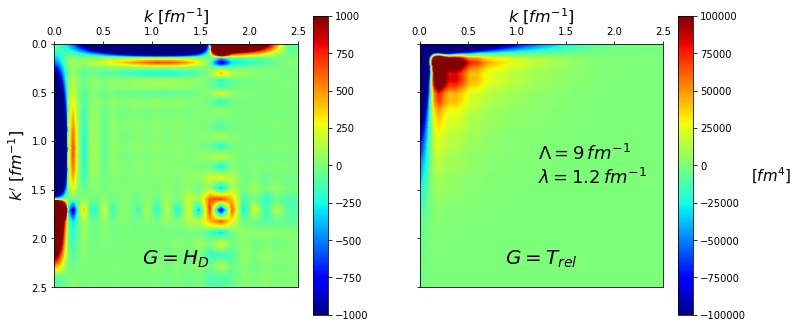
\includegraphics[width=10cm]{r2_difference_magnus_Wendt_Lamb9}
  \hspace*{0.05\textwidth}
  \caption{Difference in evolved and bare matrix elements of $\mel{k}{r^2}{k'}$ Magnus evolving to $\lambda=1.2 \, fm^{-1}$ with $G=H_D$ (left) and $G=T_{rel}$ (right). Here $\Lambda=9 \, fm^{-1}$ and $k_{max}=6$. (Note the difference in color bar scales.)}
  \label{fig:r2_difference_magnus_Wendt_Lamb9}
\end{figure}
%
\begin{figure}[H]
  \captionsetup{singlelinecheck=false,justification=raggedright}
  \centering
  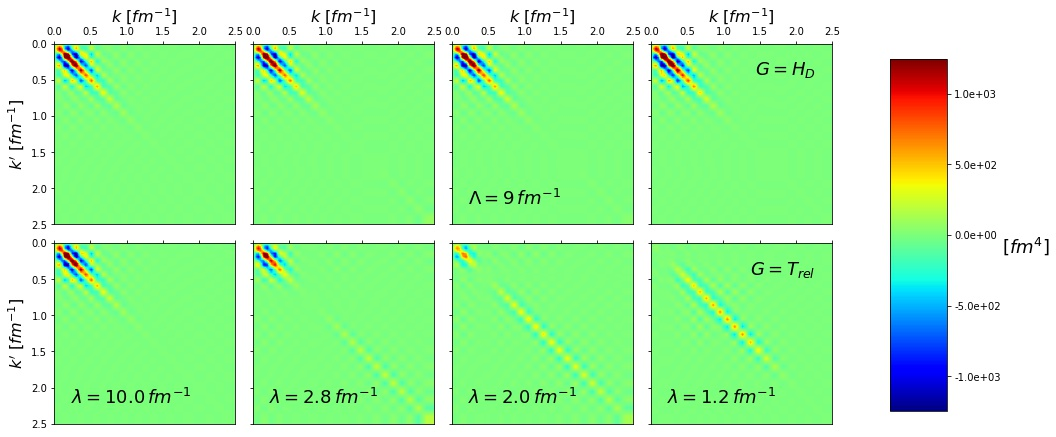
\includegraphics[width=14cm]{r2_integrand_contours_magnus_Wendt_Lamb9}
  \hspace*{0.05\textwidth}
  \caption{Integrand of $\bra{\Psi}\ket{k} \mel{k}{r^2}{k'} \bra{k'}\ket{\Psi}$ Magnus evolving the wave function in $\lambda$ right to left with $G=H_D$ (top) and $G=T_{rel}$ (bottom). Here $\Lambda=9 \, fm^{-1}$, $k_{max}=6$, and the operator $r^2$ is un-evolved.}
  \label{fig:r2_integrand_contours_srg_Wendt_Lamb9}
\end{figure}

	
%%%%%%%%%%%%%%%%%%%%%%%%%%%%%%%%%%%%%%%%%%%%%%%%%%%%%%%%%%%%%%%%%%%%%%%%%
\section{Conclusion}
\label{sec:conclusion}


\noindent{-- Summarize.}
\\
-- Where does the Magnus implementation differ from the SRG result?
\\
-- Connection to the IMSRG intruder state problem.
\\
-- Outlook.


%%%%%%%%%%%%%%%%%%%%%%%%%%%%%%%%%%%%%%%%%%%%%%%%%%%%%%%%%%%%%%%%%%%%%%%%%


\bibliography{tropiano_srg} 

\end{document}